\section{Generic Dataflow Management}

\subsection{A More General Dataflow Model}

MapReduce consists fo a map phase, followed by shuffling, followed by a reduce phase. Because reduce and map are essentially doing the same, one could also say that MapReduce follows the schema Map$\rightarrow$Shuffle$\rightarrow$Map. One can abstract away the partition and consider the nput, intermediate input and output as blackboxes that these phases act on.

\subsection{Resilient Distributed Datasets}
The first idea behind generic dataflow processing is to allow the dataflow to be arranged in any distributed acyclic graph (DAG), like so:

\begin{figure}[h]
    \centering
    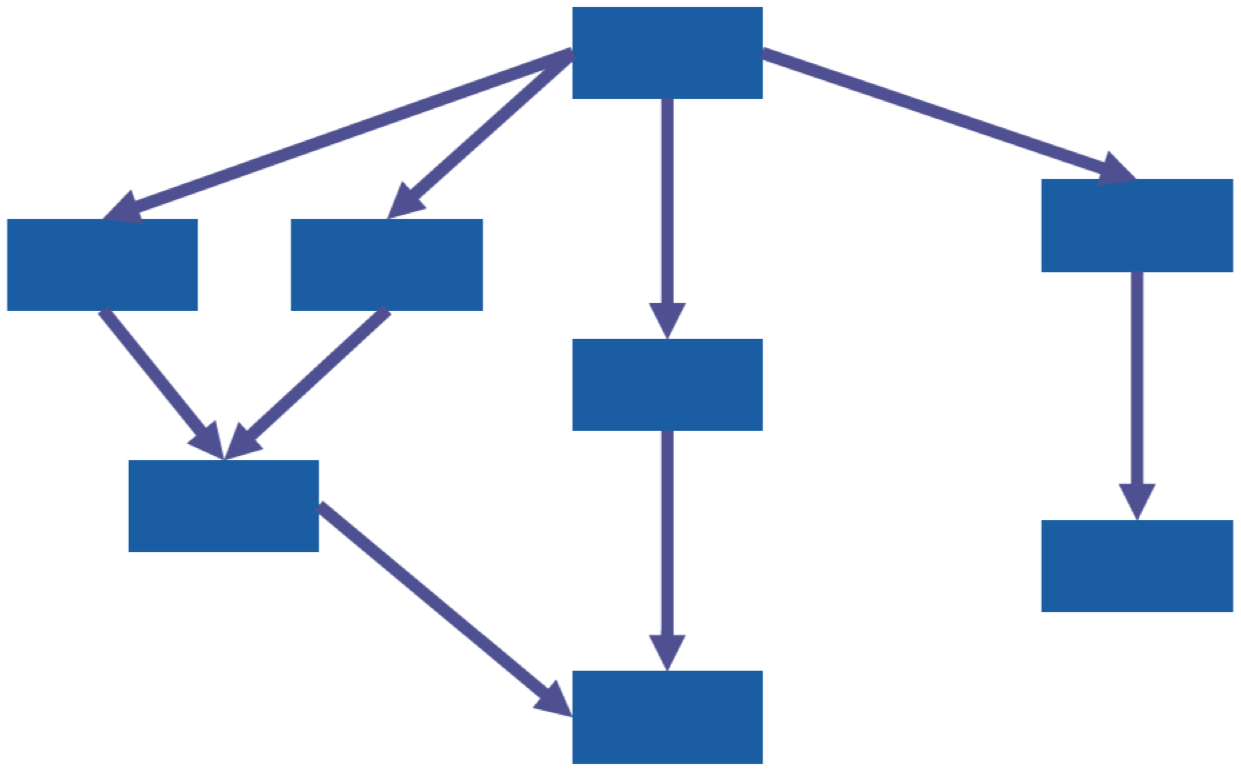
\includegraphics[width=0.4\textwidth]{Figures/DAGSpark.png}
    \caption{Dataflow in any DAG.}\label{fig:DAG}
\end{figure}

All the rectangular nodes in the above graph correspond to intermediate data. They are called resilient distributed datasets, or in short, RDDs. Resilient means that they remain in memory or on disk on a "best effort" basis, and can be recomputed if need be. Distributed means that, just like the collections of key-value pairs in MapReduce, they are partitioned and spread over multiple machines.

A major difference with MapReduce, though, is that RDDs need not be collections of pairs. In fact, RDDs can be (ordered) collections of just about anything. The only constraint is that the values within the same RDD share the same static type, which does not exclude the use of polymorphism.

Since a key-value pair is a particular example of possible value, RDDs are a generalization of the MapReduce model for input, intermediate input and output.


\subsection{The RDD Lifecycle}

\subsubsection{Creation}
RDDs can be created by reading a dataset from the local disk, or from cloud storage, or from a distributed file system, or from a database source, or directly on the fly from a list of values residing in the memory of the client using Apache Spark.

\subsubsection{Transformation}
RDDs can be transformed into other RDDs. Mapping or reducing, in this model, become two very specific cases of transformations. However, Spark allows for many more kinds of transformations. This also includes transformations with several RDDs as input (think of joins or unions in the relational algebra, for example).

\subsubsection{Action}
RDDs can also undergo a final action leading to making an output persistent. This can be by outputting the contents of an RDD to the local disk, to cloud storage, to a distributed file system, to a database system, or directly to the screen of the user.

\subsubsection{Lazy Evaluation}
The evaluation is lazy! Creations and transformations on their own do nothing. Only if an action is triggered, will the mappings like creations and transformations be computed. Especially, only those will be calculated that are needed for the action.


\subsection{Transformations}

\subsubsection{Unitary Transformations}

Unitary transformations are transformations that take only one RDD as their input.

\paragraph{Filter Transformation:} Provided a predicate function taking a value and returning a boolean, the Filter transformation returns the subset of its inputs that satisfy the predicate, preserving the relative order.

\paragraph{Map Transformation:} Provided a function taking a value and returning another value, the Map transformation returns the list of values obtained by applying this function to each value in the input.

\paragraph{flatMap Transformation:} Privided a function taking a value and returning zero, one or more values, the flatMap Transformation returns the list of values obtained by applying this function to each value in the input, flattening the obtained values (i.e. the information on which values came from the same input value is lost). The flatMap transformation corresponds to the MapReduce map phase.

\paragraph{Distinct Transformation} eliminates duplicates in the input. You either supply a comparison function, or you make sure that the class (type) of the input values implements the appropriate comparable interface.

\paragraph{Sample Transformation} samples the input to a smaller list. It is possible to specify the sampling percentage.


\subsubsection{Binary Transformations}

Binary transformations take two RDDs as inputs.

\paragraph{Union:} You concatenate two RDDs.

\paragraph{Intersection:} You filter the values that are present in both RDDs and create a new RDD out of these values.

\paragraph{Subtract:} Only keep the elements from the left RDD that do not appear in the right RDD.

\paragraph{Cartesian Product:} Looks for all possible combinations of the values in the left and right RDD and outputs pairs of these values. By default, Spark will not let you do this because it could yield enormous files.

\subsubsection{Pair Transformation}

\paragraph{key Transformation} returns a new RDD with only the keys.

\paragraph{value Transformation} returns a new RDD with only the values.

\paragraph{reduceByKey Transformation} given a binary operator, this function applies this function to all key values pairs with the same key. The reduceByKey transformation corresponds to the reduce phase of MapReduce.

\paragraph{groupByKey Transformation}  groups all key-value pairs by key, and outputs a single key-value for each key, where the value is an array (or list) of all the values that were associated with this key in the input.

\paragraph{sortByKey Transformation} given the specification of an order or comparison operator on the key type, the sortByKey transformation outputs the same pairs as in the input RDD, but reordered by key.

\paragraph{mapValues Transformation} similar to the map transformation, except that the map function is only applied to the value.

\paragraph{join Transformation} acts on two RDDs or key-value pairs. It matches pairs on both sides that have the same key and outputs, for each match, an ouput pair with that shared key and a tuple with the two valuse from each side. If there are multiple values with the same key on any side (or both), then all possible combinations are output.

\paragraph{subtractByKey:} outputs all pairs of the left, except those who have a key present on the right.


\subsection{Actions}

\subsubsection{Gathering output locally}

\paragraph{collect action} downloads all values of an RDD on the client machine and outputs them as a (local) list.

\paragraph{count action} computes (in parallel) the total number of values in the input RDD.

\paragraph{countByValue action} computes the total number of occurrence of each distinct value in the input RDD. The output is a python dictionary with the value as the key and the number of occurrences as the value.

\paragraph{take action} returns, as a local list, the first $n$ values in the input RDD.

\paragraph{top action} returns, as a local list, the last $n$ values from the input RDD.

\paragraph{takeSample action} returns, as a local list $n$ randomly picked values from the input RDD.

\paragraph{reduce action} given a (normally associative and commutative) binary operator, the reduce action invokes this operator on all values of the input RDD and outputs the resulting value.


\subsubsection{Actions on Pair RDDs}

(you can have repeating keys)

\paragraph{countByKey action} outputs, locally as a python dictionary, each key together with the number of values in the input that are associated with this key.

\paragraph{lookup action} outputs, locally, the value or values associated with a specific key.


\subsection{Physical Architecture}

There are two kinds of transformations: narrow-dependency transformations (not spaghetti-y) and wide-dependency transformations (spaghetti-y).

\subsubsection{Narrow-dependency Transformations}
Here, the computations of each output value involves a single input value. Thus, it is comparable to the map phase of MapReduce, and is easily parellelizable. Per default, there is one task per HDFS block.

The sequential calls of the transformation function on each input value within a single partitoin is called a task. Just like MapReduce, the tasks are assigned to slots. These slots correspond to cores within YARN containers. YARN containers used by Spark are called executors. The processing of the tasks is sequential within each executor, and tasks are executed in parallel across executors. A queue of unprocessed tasks is maintained, and everytime a slot is done, it gets a new task. When all tasks have been assigned, the slots who are done become idle and wait for all others to complete.

\subsubsection{Chains of narrow-dependency Transformations}

Consider the case of a chain of several narrow-dependency transformations, executed in turn (\cref{subfig:NDchain}). Naively, one could expect the execution to look like \cref{subfig:NaiveEx}. However, this would be very ineffienent because it requires shipping intermediate data over the network. But if all transformations are narrow-dependency transformations, it is possible to chain them without having data leaving the machines (\cref{subfig:EffEx}).

In fact, on the physical level, the physical calls of the underlying map/filter/etc functions are directly chained on each input value to directly produce the corresponding final, output value, meaning that the intermediate RDDs are not even materialized anywhere and exist purely logically. This means in particular that there is a single set of tasks, one for each partition of the input, for the entire chain of transformations. (\cref{subfig:BetterNDChain})

Such a chain of narrow-dependency transformations executed efficiently as a single set of tasks is called a stage, which would correspond to what is called a phase in MapReduce.

\begin{figure}[h]
    \centering
    \begin{subfigure}{0.47\textwidth}
        \centering
        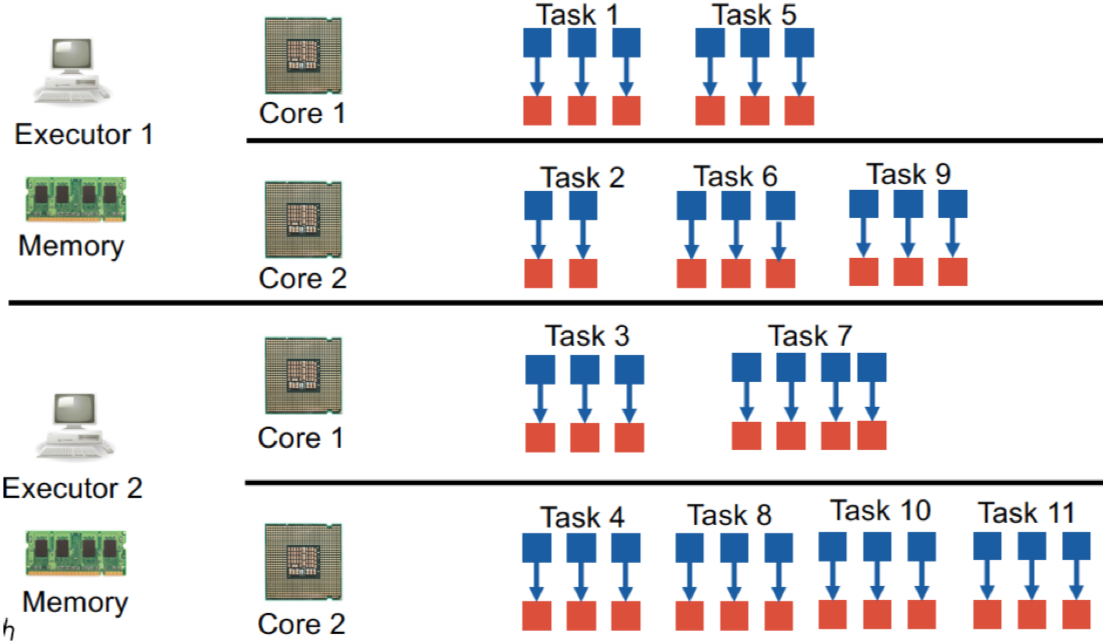
\includegraphics[width=\textwidth]{Figures/ChainTransformations.jpeg}
        \caption{Chain of several narrow-dependency transformations.}\label{subfig:NDchain}
    \end{subfigure}
    \hfill
    \begin{subfigure}{0.47\textwidth}
        \centering
        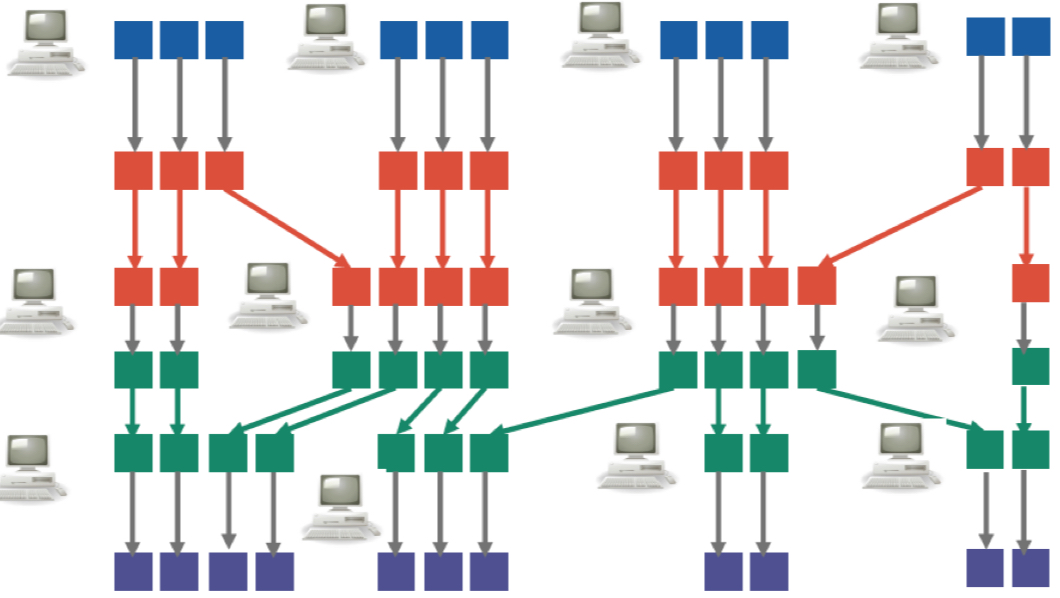
\includegraphics[width=\textwidth]{Figures/NaiveExecutionChain.jpeg}
        \caption{Naive Execution.}\label{subfig:NaiveEx}
    \end{subfigure}
    \begin{subfigure}{0.47\textwidth}
        \centering
        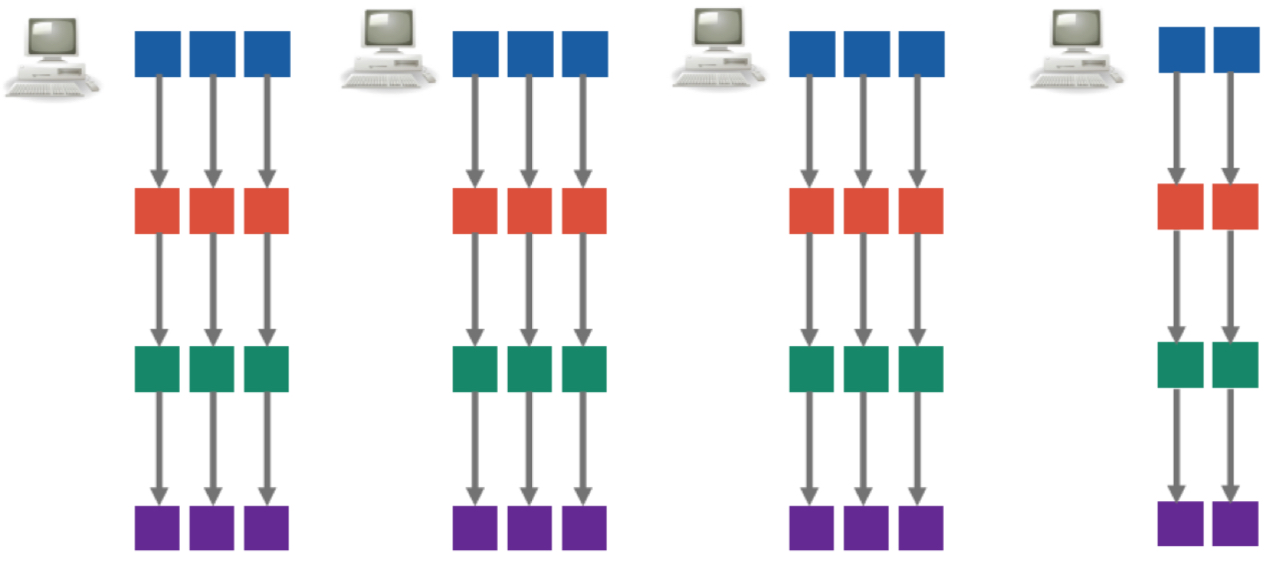
\includegraphics[width=\textwidth]{Figures/EfficientExecutionChain.jpeg}
        \caption{Efficient Execution.}\label{subfig:EffEx}
    \end{subfigure}
    \hfill
    \begin{subfigure}{0.47\textwidth}
        \centering
        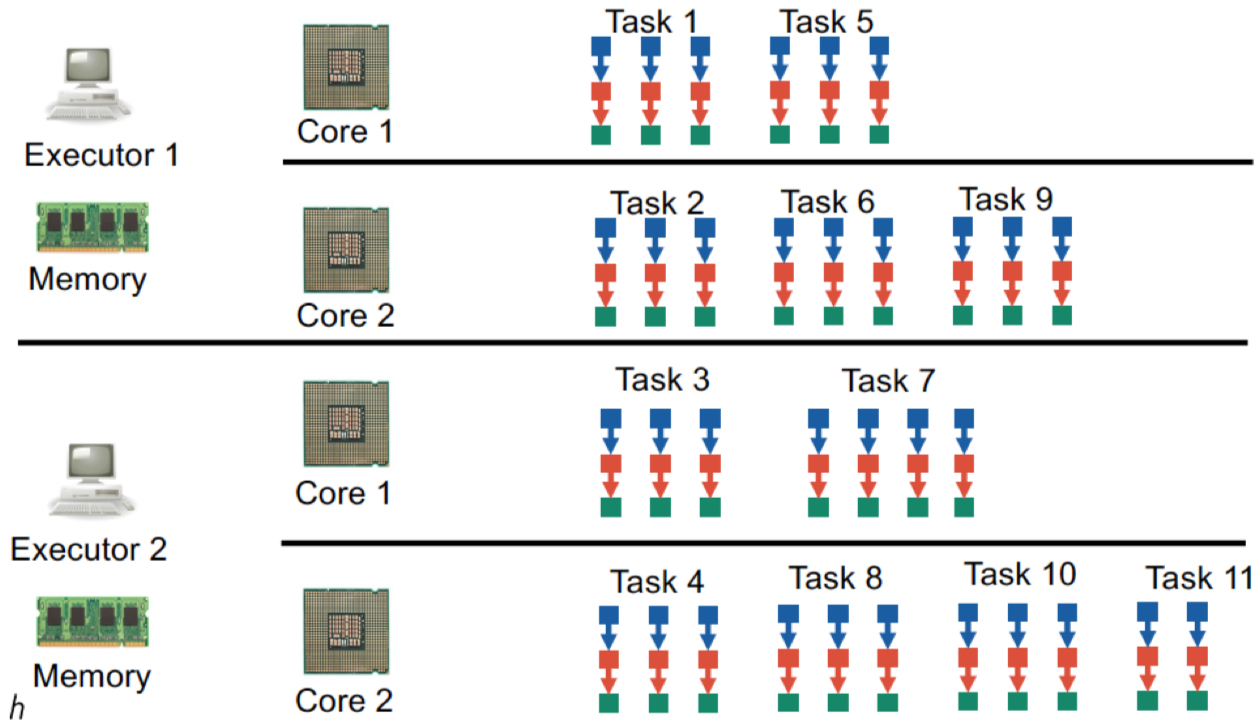
\includegraphics[width=\textwidth]{Figures/BetterNDChain.jpeg}
        \caption{Parallelized Executions.}\label{subfig:BetterNDChain}
    \end{subfigure}
    \caption{Narrow-dependency Transformations}\label{fig:NDTransfo}
\end{figure}

\subsubsection{Physical Parameters}
Users can parameterize how many executors there are, how many cores there are per executor and how much memory per executor. E.g.

\begin{lstlisting}[style=Java]
spark-submit
    --num-executors 42
    --executor-cores 2
    --executor-memory 3G
    my-application.jar
\end{lstlisting}

\subsubsection{Shuffling}
Wide-dependency transformations involve a shuffling of the data over the network, so that the data necessary to compute each partition of the output RDD is physically at the same location. Thus, on the high-level of a job, the physical execution consists of a sequence of stages, with shuffling happening everytime a new stage begins (\cref{subfig:stageshuffleseq})

Even though one can imagine a physical implementation in which two stages are executed at the same time on two sub-parts of the cluster, a more typical setting is a linear succession of stages on the physical level. (\cref{subfig:parallStageShuffleSeq})

\begin{figure}[h]
    \centering
    \begin{subfigure}{0.47\textwidth}
        \centering
        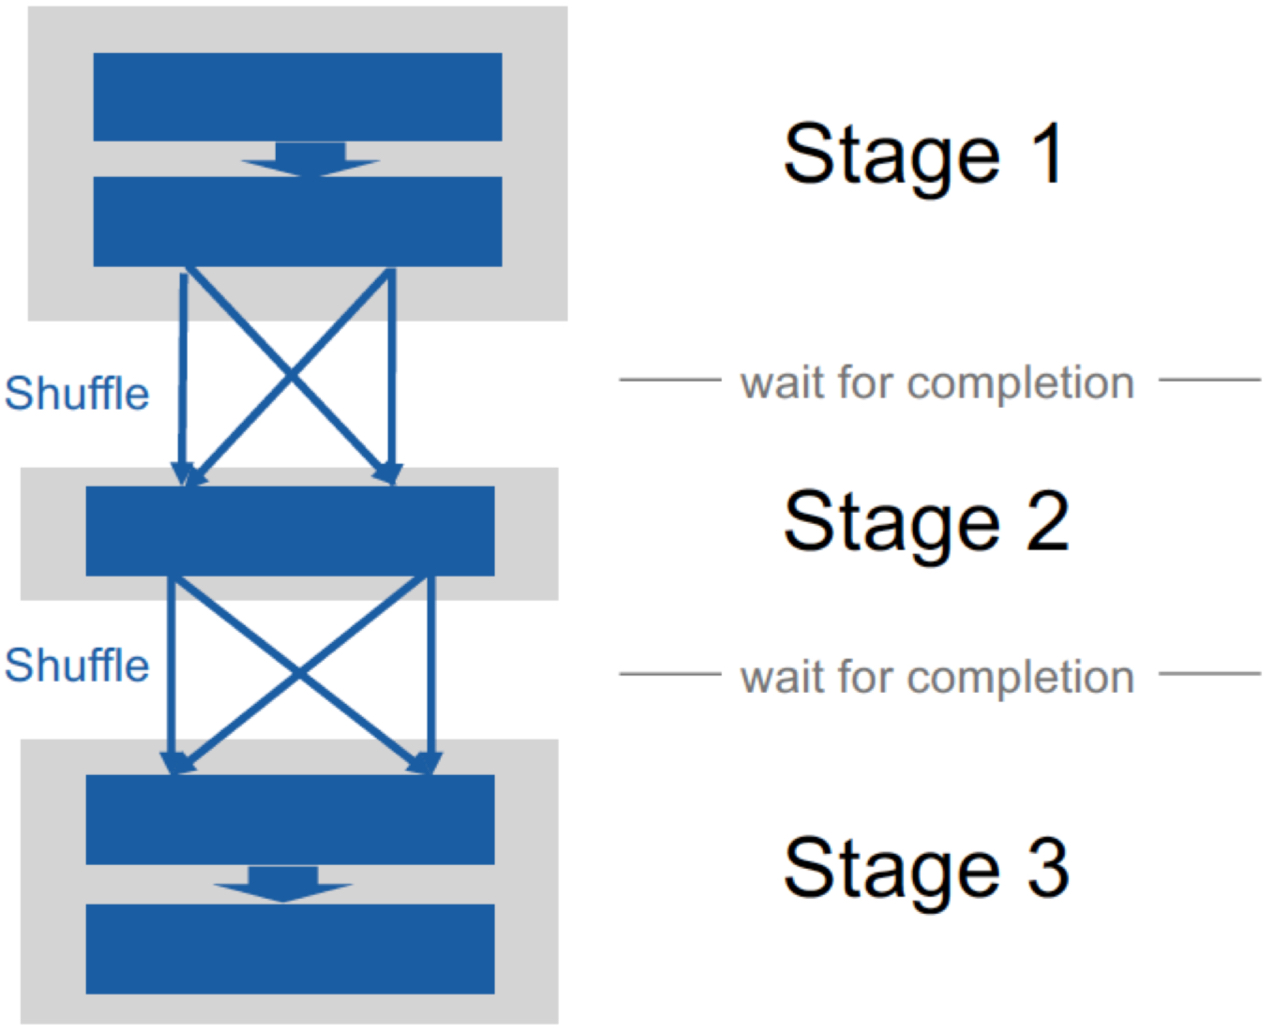
\includegraphics[width=0.8\textwidth]{Figures/StageShuffleSequence.jpeg}
        \caption{Sequence of Stages and Shuffles.}\label{subfig:stageshuffleseq}
    \end{subfigure}
    \hfill
    \begin{subfigure}{0.48\textwidth}
        \centering
        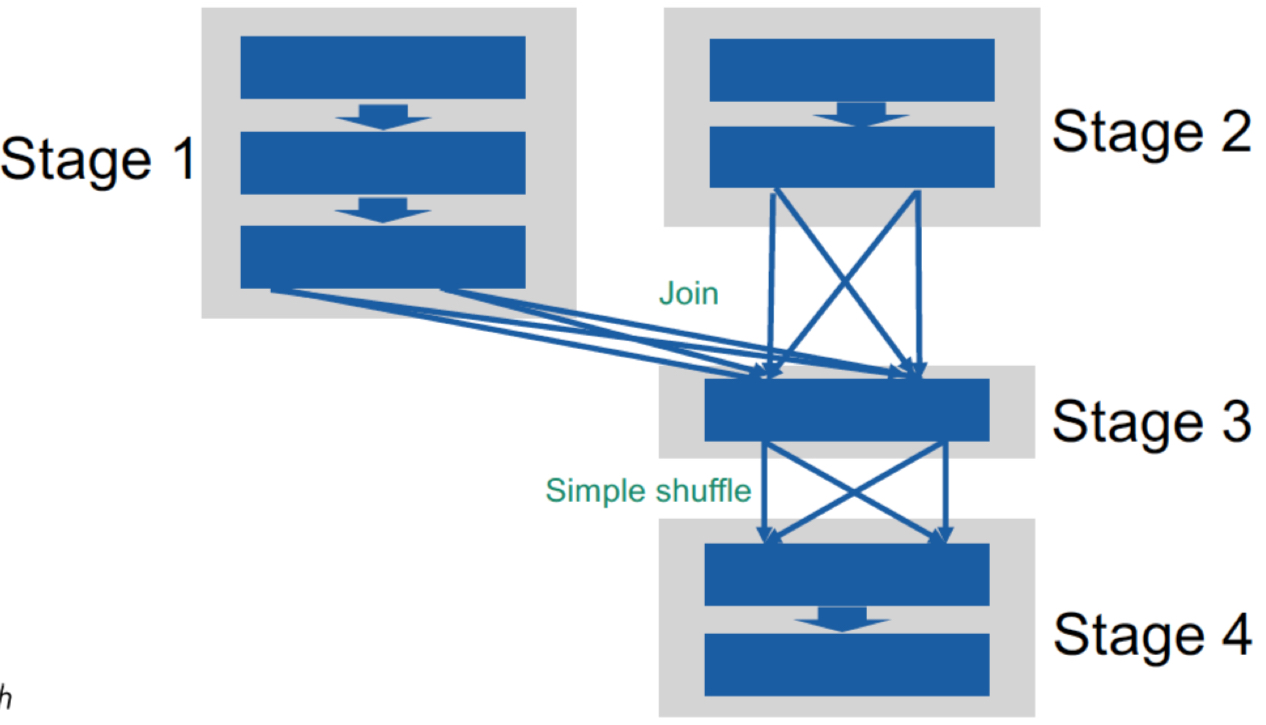
\includegraphics[width=\textwidth]{Figures/ParellelStageShuffleSeq.jpeg}
        \caption{Parallel Sequence of Stages and Shuffles.}\label{subfig:parallStageShuffleSeq}
    \end{subfigure}
    \caption{Sequence of Stages and Shuffles.}
\end{figure}

\subsubsection{Optimization}

\paragraph{Pinning RDDs}
In some cases, several actions might share subgraphs of the DAG. It makes sense, then, to “pin” the intermediate RDD by persisting it. It is possible to ask for persistence in memory and/or on disk.

\paragraph{Pre-Partitioning}
Shuffle is needed to bring together the data that is needed to jointly contribute to individual output values. If, however, Spark knows that the data is already located where it should be, then shuffling is not needed.

\subsubsection{Summary}
Tasks, Transformations, Stages and Jobs relate as can be seen in \cref{fig:Terminology}

\begin{figure}[h]
    \centering
    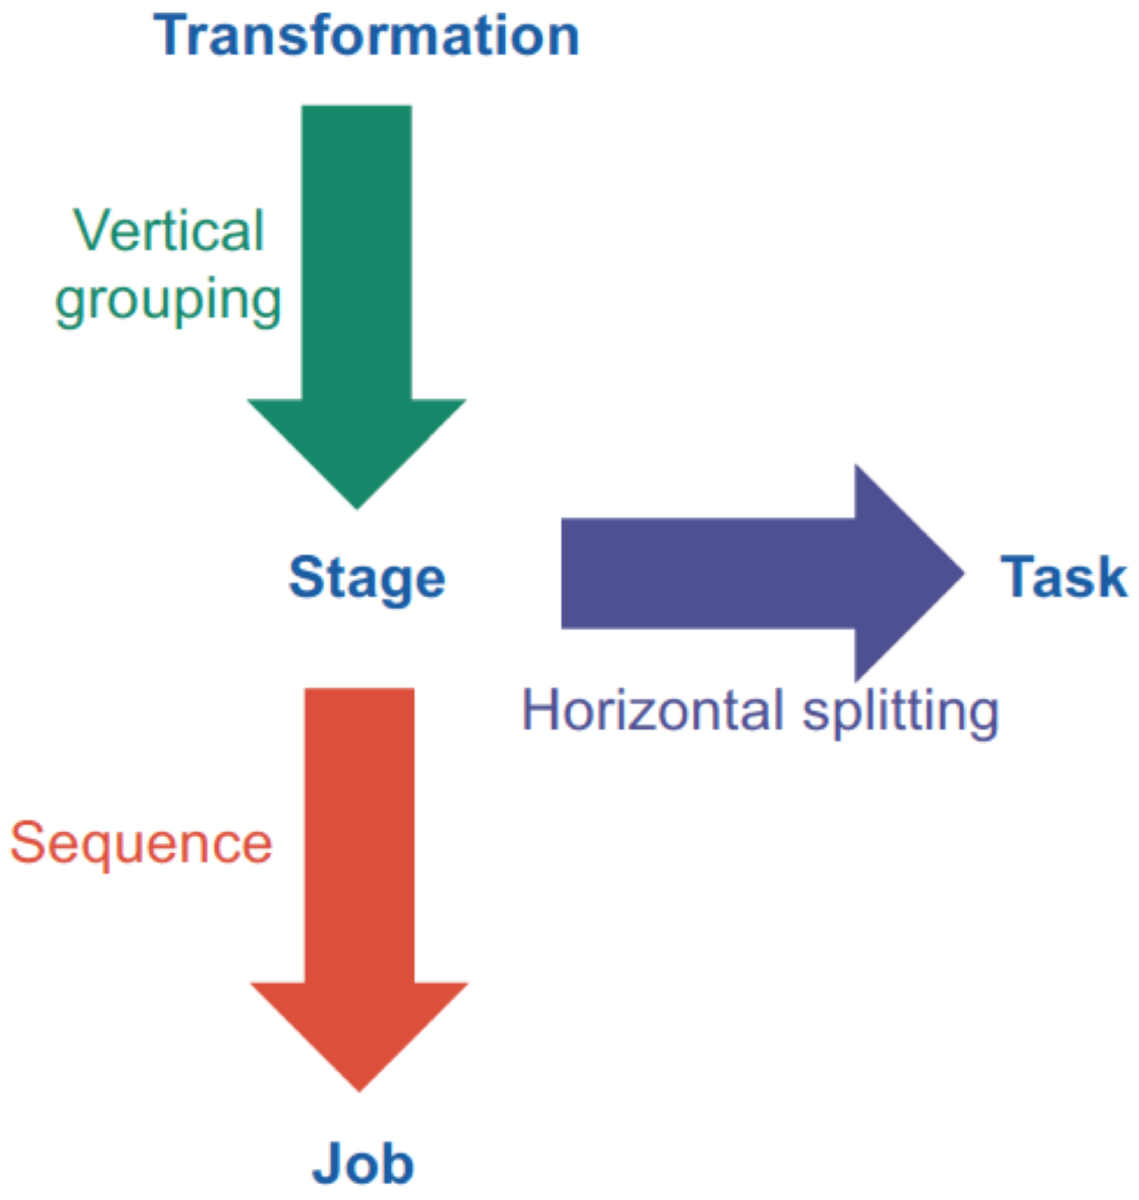
\includegraphics[width=0.4\textwidth]{Figures/Terminology.jpeg}
    \caption{Terminology}\label{fig:Terminology}
\end{figure}


\subsection{DataFrames in Spark}

\subsubsection{Data Independence}
Unlike a relational database that has everything right off-the-shelf, with RDDs, the user has to reimplement all the primitives they need.

\subsubsection{A Specific Kind of RDD}
A DataFrame can be seen as a specific kind of RDD: an RDD of rows (equivalently: tuples, records) that has relational integrity, domain integrity, but not necessarily atomic integrity. DataFrames can also be characterized as homogeneous collections of valid JSON objects (which are the rows) against a schema. It is thus only logical that, in Spark, every DataFrame has a schema.

The immediate consequence is that, in the particular case of flat rows, an RDD of (flat) rows is a relational table. Thus, it is very natural to think of SQL as the natural language to query them.

\subsubsection{Performance Impact}
DataFrames are not only useful because of the higher, more convenient, level of abstraction that they provide to the user, enhancing their productivity. DataFrames also have a positive impact on performance, because Spark can do a much better job of optimizing the memory footprint and the processing. In particular, DataFrames are stored column-wise in memory, meaning that the values that belong to the same column are stored together. Furthermore, since there is a known schema, the names of the attributes need not be repeated in every single row, as would be the case with raw RDDs. DataFrames are thus considerably more compact in memory than raw RDDs.

Generally, Spark converts Spark SQL to internal DataFrame transformation and eventually to a physical query plan. An optimizer known as Catalyst is then able to find many ways of making the execution faster, as knowing the DataFrame schema is invaluable information for an optimizer, as opposed to generic RDDs of which one knows little statically.

As an example, since the data is stored by columns, whenever Spark knows that some columns are not used by subsequent transformations and actions, it can silently drop these unused columns with no consequence. This is called “projecting away” and it is one of the most important optimizations in large-scale databases. Projecting away can even be done already at the disk level, i.e., when reading a Parquet file, it is possible to read only the columns that are actually needed, which significantly reduces the I/O bottleneck and accelerates the job.


\subsubsection{Input Formats}
Here an example of code in which a dataset is directly read as JSON. 

\begin{lstlisting}[style=neutral]
df = spark.read.json('hdfs:///dataset.json')
df.createOrReplaceTempView("dataset")
df2 = df.sql("SELECT * FROM dataset "
"WHERE guess = target "
"ORDER BY target ASC, country DESC, date DESC")
result = df2.take(10)
\end{lstlisting}

Note that Spark automatically infers the schema from discovering the JSON Lines file, which adds a static performance overhead that does not exist for raw RDDs. CSV also come with a schema discovery, although this one is optional (as by default, one can treat all values as strings). Builtin input formats can be specified, when creating a DataFrame from a dataset, with a simple method call after the read command. Non-builtin formats are supplied as a string parameter to a format() method. This is extensible and it is possible to “make” a format builtin via extension libraries.

\begin{lstlisting}[style=neutral]
df = spark.read.json("hdfs:///dataset.json")
df = spark.read.parquet("hdfs:///dataset.parquet")
df = spark.read.csv("hdfs:///dir/*.csv")
df = spark.read.text("hdfs:///dataset[0-7].txt")
df = spark.read.jdbc("jdbc:postgresql://localhost/test?user=fred&password=secret",...)
df = spark.read.format("avro").load("hdfs:///dataset.avro")
\end{lstlisting}

\subsubsection{DataFrame Column Types}
There are atomic (\cref{fig:AtomicTypes}) and structured types (\cref{fig:StructuredTypes}). As a reminder, structs have string keys and arbitrary value types and correspond to generic JSON objects, while in maps, all values have the same type. Thus, structs are more common than maps. Arrays correspond to JSON arrays.

\begin{figure}[h]
    \centering
    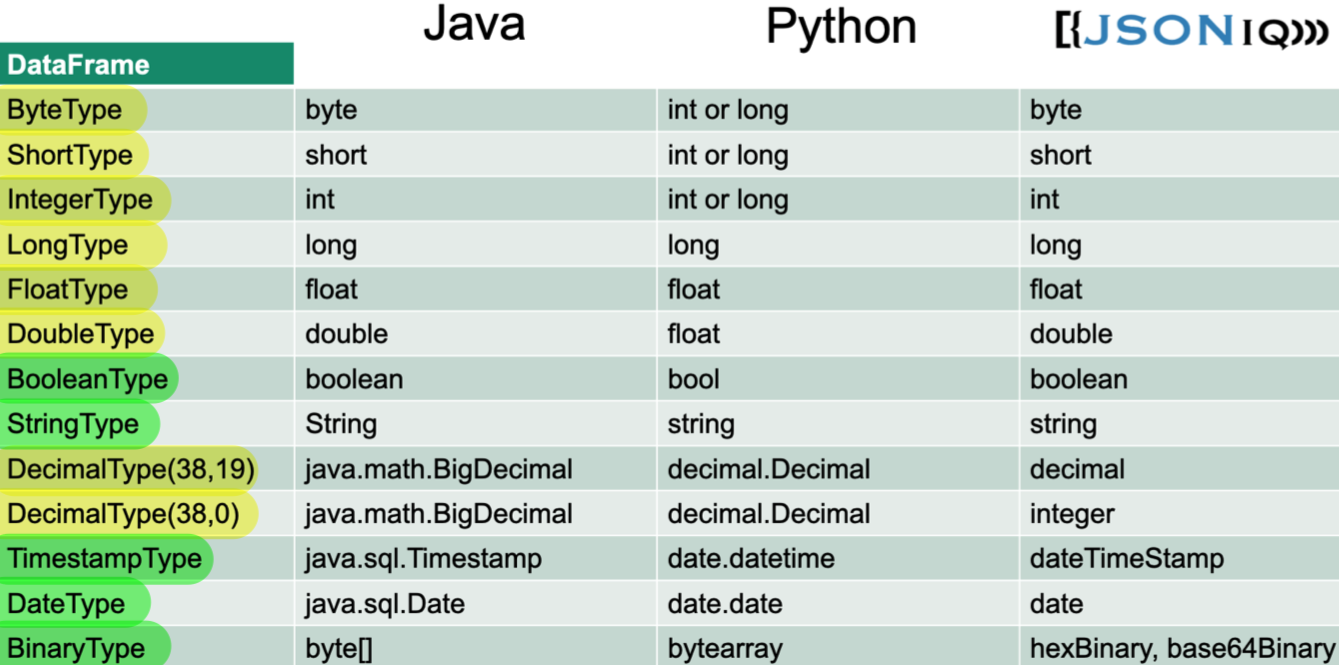
\includegraphics[width=0.8\textwidth]{Figures/DataFrameTypes.png}
    \caption{Atomic DataFrame Types. Yellow corresponds to Number types and green corresponds to non-number types (/other atomics)}\label{fig:AtomicTypes}
\end{figure}

\begin{figure}[h]
    \centering
    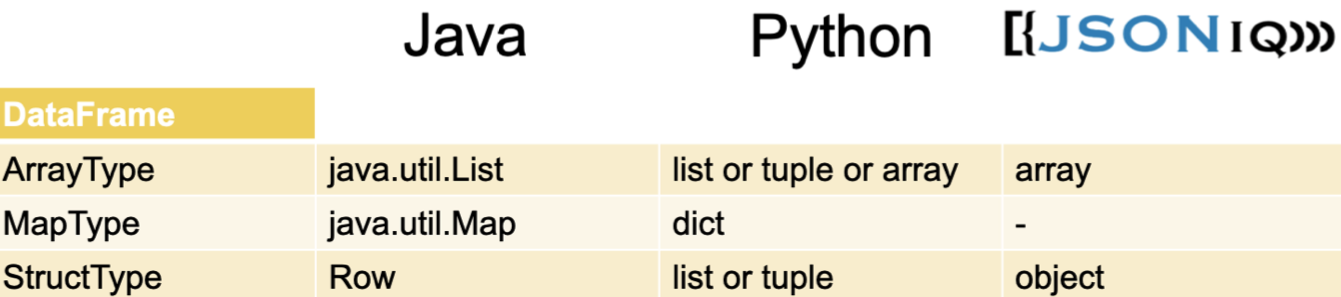
\includegraphics[width=0.7\textwidth]{Figures/DataFrameTypes2.png}
    \caption{Structured DataFrame Types.}\label{fig:StructuredTypes}
\end{figure}

\subsubsection{The Spark SQL Dialect}

We mentioned that Spark SQL is a dialect of SQL. Spark SQL has a few limitations (i.e., there is no OFFSET clause) but also comes with a few convenient extensions, in particular to deal with nested data.

\begin{lstlisting}[style=sql]
SELECT first_name, last_name
FROM persons
WHERE age >= 65
GROUP BY country
HAVING COUNT(*) >= 1000
ORDER BY country DESC NULLS FIRST
LIMIT 100
\end{lstlisting}

GROUP BY and ORDER BY will trigger a shuffle in the system, even though this can be optimized as the grouping key and the sorting key are the same.

The SORT BY clause can sort rows within each partition, but not across partitions, i.e., does not induce any shuffling.

The DISTRIBUTE BY clause forces a repartition by putting all rows with the same value (for the specified field(s)) into the same new partition.

\begin{minipage}{0.45\textwidth}
\begin{lstlisting}[style=sql]
SELECT first_name, last_name
FROM persons
WHERE age >= 65
GROUP BY country
HAVING COUNT(*) >= 1000
SORT BY country DESC NULLS FIRST
\end{lstlisting}
\end{minipage}
\hfill
\begin{minipage}{0.45\textwidth}
\begin{lstlisting}[style=sql]
SELECT first_name, last_name
FROM persons
WHERE age >= 65
GROUP BY country
HAVING COUNT(*) >= 1000
DISTRIBUTE BY country
\end{lstlisting}
\end{minipage}

It is possible to use both SORT and DISTRIBUTE, but this is equivalent to the use of another clause, CLUSTER BY:

\begin{minipage}{0.45\textwidth}
\begin{lstlisting}[style=sql]
SELECT first_name, last_name
FROM persons
WHERE age >= 65
GROUP BY country
HAVING COUNT(*) >= 1000
SORT BY country DESC NULLS FIRST
DISTRIBUTE BY country
\end{lstlisting}
\end{minipage}
\hfill
\begin{minipage}{0.45\textwidth}
\begin{lstlisting}[style=sql]
SELECT first_name, last_name
FROM persons
WHERE age >= 65
GROUP BY country
HAVING COUNT(*) >= 1000
CLUSTER BY country
\end{lstlisting}
\end{minipage}

Spark SQL also comes with language features to deal with nested arrays and objects.
First, nested arrays can be navigated with the explode() function, like so:

\begin{figure}[h]
    \centering
    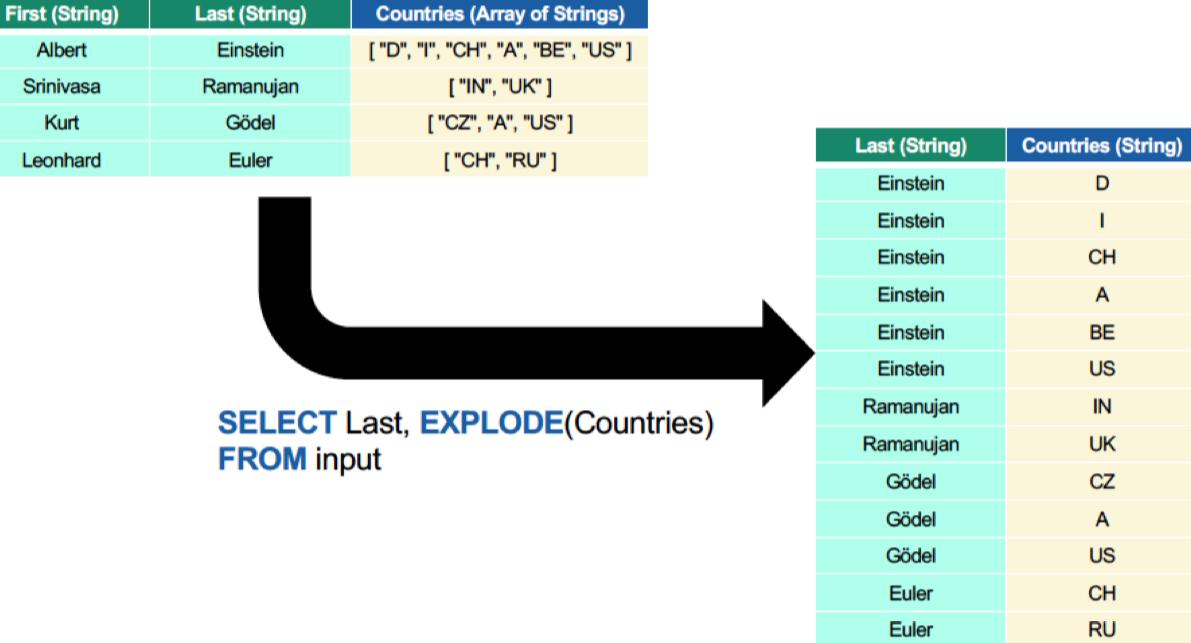
\includegraphics[width=0.8\textwidth]{Figures/Explode.png}
    \caption{Explode}\label{fig:Explode}
\end{figure}

Explode() cannot deal with all use cases, though, which is why there is another, more generic construct known as LATERAL VIEW. A lateral view can be intuitively described this way: the array mentioned in the LATERAL VIEW clause is turned into a second, virtual table with the rest of the original table is joined. The other clauses can then refer to columns in both the original and second, virtual table. This yields the same result as can be seen in \cref{fig:Explode}.  Lateral views are more powerful and generic than just an explode() because they give more control, and they can also be used to go down several levels of nesting, like in \cref{fig:LatView}.

\begin{figure}[h]
    \centering
    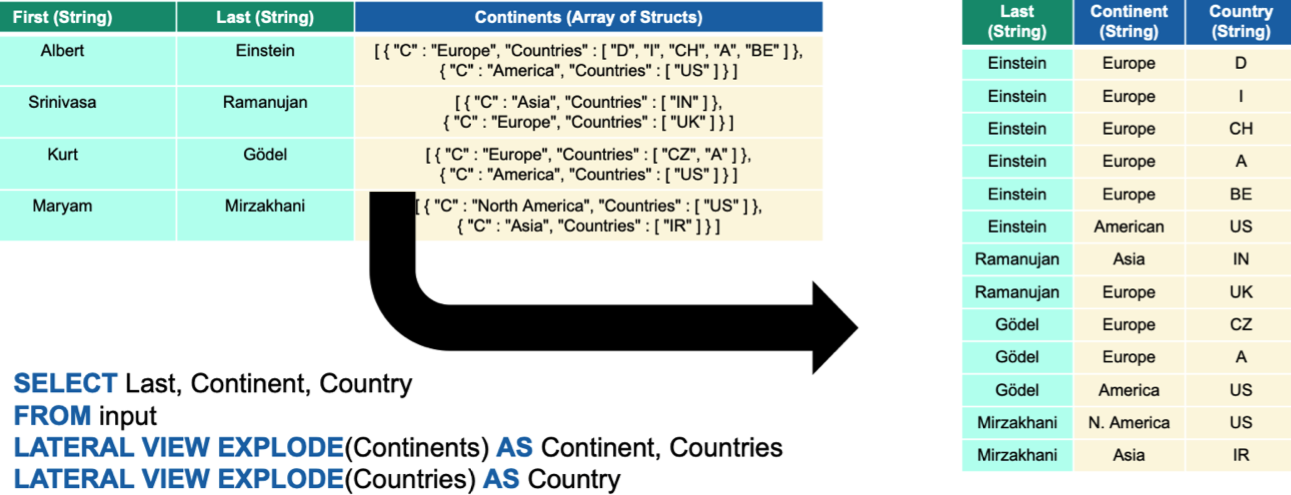
\includegraphics[width=0.8\textwidth]{Figures/LateralViewExplode.png}
    \caption{Lateral View}\label{fig:LatView}
\end{figure}

It is also possible to navigate and “unnest” nested structs (objects) using dots, like in \cref{fig:Unnest}.

\begin{figure}[h]
    \centering
    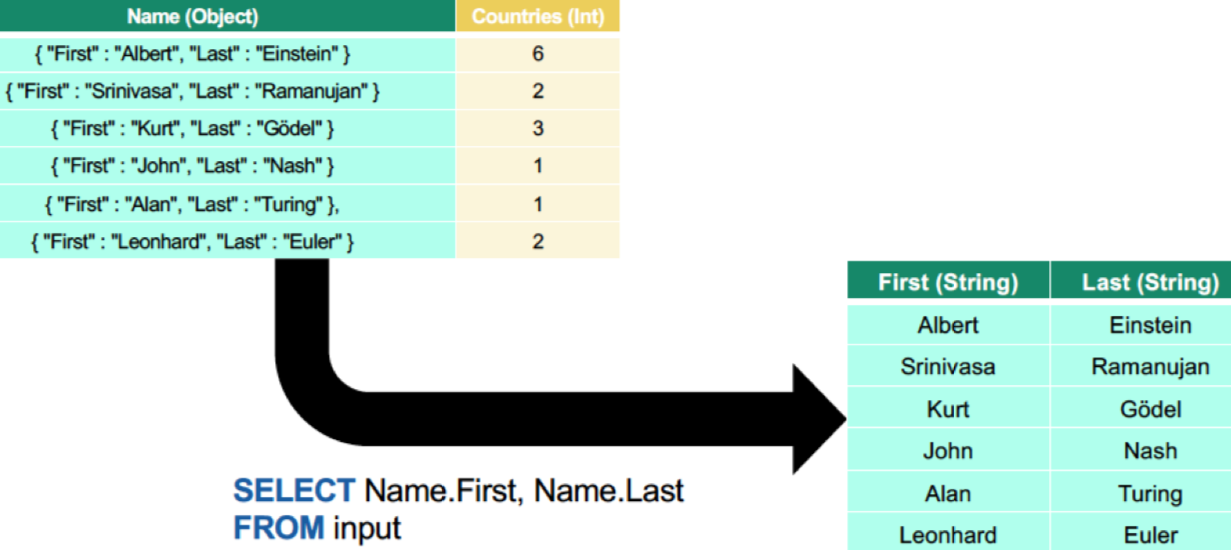
\includegraphics[width=0.8\textwidth]{Figures/UnnestStructs.png}
    \caption{Unnest nested structs.}\label{fig:Unnest}
\end{figure}

DataFrames and Spark SQL do support data that is not in first normal form, but they do not support at all data that does not fulfill relational integrity or domain integrity. It is possible to read as input a JSON Lines dataset with inconsistent value types in the same columns, however the schema discovery phase will simply result in a column with type “string”, which puts all the burden of dealing with the polymorphism of the column to the end user.


\subsubsection{DataFrames and RDDs}
Under the hood, when creating dataframes, spark is storing them as RDDs. But you can also do it explicitely. If you have a dataframe, you can force-convert it to an RDD and vice versa. But to turn an RDD into a dataframe, you need a schema. See \cref{lst:DFaRDD}.

\vspace{1\baselineskip}

\begin{lstlisting}[style=neutral,caption={DataFrames and RDDs},label={lst:DFaRDD}]
# Create an RDD file from a DataFrame
rdd = df.rdd

# Create a DataFrame from an RDD file
df = rdd.toDF()
# or
df = sc.createDataFrame(rdd,schema)
\end{lstlisting}
